\documentclass[12pt,a4paper]{article}
\usepackage[utf8]{inputenc} %polskie znaki
\usepackage[T1]{fontenc}	%polskie znaki
\usepackage{amsmath}		%matematyczne znaczki :3
\usepackage{enumerate}		%Dodatkowe opcje do funkcji enumerate
\usepackage{geometry} 		%Ustawianie marginesow
\usepackage{graphicx}		%Grafika
\usepackage{wrapfig}		%Grafika obok textu
\usepackage{float}			%Allows H in fugire
\pagestyle{empty} 			%usuwa nr strony

\newgeometry{tmargin=2cm, bmargin=2cm, lmargin=2cm, rmargin=2cm} 

\begin{document}
	\begin{center}
		\LARGE Rachunek prawdopodobieństwa - test
	\end{center}
	\vspace{1.5cm}
	\begin{flushright}
		\textbf{1 TERMIN}
	\end{flushright}
	\begin{tabular}{p{13cm} r}
		Imię i nazwisko: ............................................................................
		&[....../30pkt]\\ 
		\vspace{0.5cm}
	\end{tabular}
	\begin{enumerate}[1.]
		\item  \begin{tabular}{p{13cm} r}
			Oblicz ile jest liczb 9-cyfrowych, w których pierwsza cyfra jest liczbą parzystą, trzy ostatnie są takie same i cyfra "7" występuje dokładnie raz. &[3pkt]\\ 
		\end{tabular}
		
		\item  \begin{tabular}{p{13cm} r}
			Farmer Donald uprawia w ogródku warzywa. Do dyspozycji ma 4 doniczki różnych kolorach (czerwoną, białą, żółtą i zieloną). W każdej doniczce może posadzić jedno z 9 różnych nasion kwiatów (nasion ma bardzo dużo). Oblicz na ile sposobów Donald może zasadzić te kwiaty w tych doniczkach.  &[2pkt]\\ 
		\end{tabular}
	
		\item  \begin{tabular}{p{13cm} r}
			Ania pracuje w przedszkolu. Pewnego dnia miała pod opieką ośmioro dzieci. Z racji, iż tego dnia był dzień dziecka, to każdego z tego obecnych dnia dzieci obdarowywała jednym z dwunastu unikalnych lizaków. Na ile sposobów Ania może rozdać dzieciom lizaki?  &[2pkt]\\ 
		\end{tabular}
	
		\item \begin{tabular}{p{13cm} r}
			Młoda para wybiera menu na ich wesele. Firma organizująca to wesele zaproponowała 10 różnych dań. Na ile sposobów para młoda może wybrać dania, jeżeli muszą się zdecydować na 3 dania podczas weselnej kolacji?	  &[2pkt]\\ 
		\end{tabular}
	
		\item  \begin{tabular}{p{13cm} r}
			Do kolejki z roller coastera wchodzi 10 osób (w tym Arek i Barbara) - (zobacz rysunek). &[4pkt]\\ 
		\end{tabular}
		
		\begin{figure}[h]
			\centering
			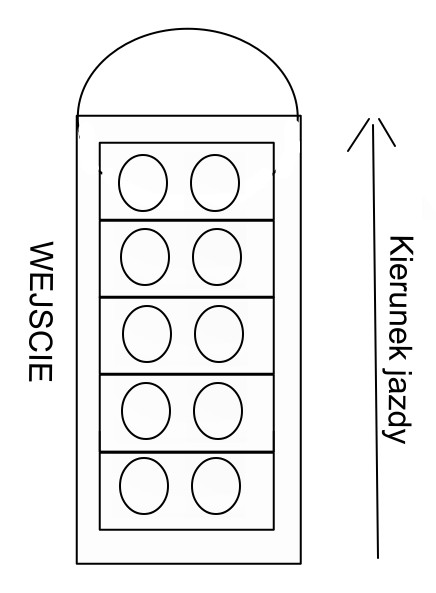
\includegraphics[scale=0.4]{rpt2.jpeg}
		\end{figure}
		Oblicz na ile sposobów mogą wsiąść te osoby:
		\begin{enumerate}[a)]
			\item dowolnie
			\item tak aby Arek i Barbara siedzieli obok siebie (czyli w tym samym rzędzie).
			\item tak aby Arek lub Barbara byli z samego przodu.
			\item tak aby Arek siedział od strony wejścia do kolejki, a Barbara w ostatnim rzędzie.
		\end{enumerate}
	

		
		\newpage
		
		
		
		\item \begin{tabular}{p{13cm} r}
			Pewna klasa organizuje loterie polegającą na wyciąganiu losów (bez zwracania). W loteri jest 160 losów przegrywających i 40 wygrywających. Oblicz prawdopodobieństwo wygrania (czyli wylosowania przynajmniej jednego losu wygrywającego) przez pewną osobę, która wyciąga dwa losy.	  &[3pkt]\\ 
		\end{tabular}
		
		\item \begin{tabular}{p{13cm} r}
			Zdarzenie losowe polega na wyciągnięciu z urny, w której są 3 kule białe, 2 czarne i 5 zielonych \textbf{jednej kuli}. Następnie, jeśli wyciągniemy:	  &[6pkt]\\ 
		\end{tabular}
		
		\begin{itemize}
			\item kulę białą - losujemy z urny, w której są 2 kule czarne i 3 zielone
			\item kulę czarną - losujemy z urny, w której są 4 kule białe i 1 zielona
			\item kulę zieloną - losujemy z urny, w której są 2 kule białe i 3 czarne.
		\end{itemize}
		
		\begin{figure}[h]
			\centering
			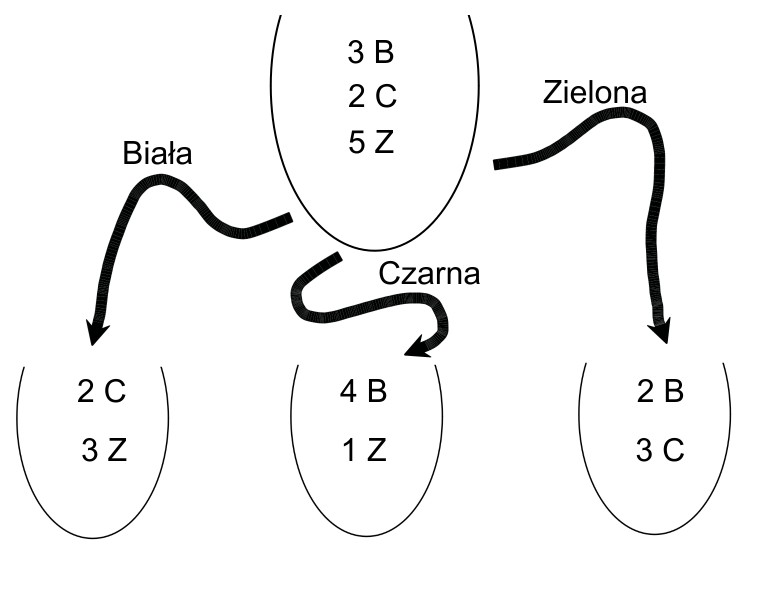
\includegraphics[scale=0.4]{rpt1.jpeg}
		\end{figure}
		
		Oblicz prawdopodobieństwo, że
		
		\begin{enumerate}[a)]
			\item za drugim razem zostanie wylosowana kula koloru zielonego.
			\item zostanie przynajmniej raz wylosowana kula czarna.
			\item w żadnym losowaniu nie zostanie wylosowana kula biała.
		\end{enumerate}
		
		
		\item  \begin{tabular}{p{13cm} r}
			Pewna pizzeria "5 na 15" tworzy pizze w dość nietypowy sposób. Klient nigdy nie wybiera sobie składników które trafiają na zamówioną przez niego pizzę, lecz wybierane jest losowo 5 spośród 15 składników ustalonych przez pizzerie. Romek niestety nie lubi ananasa, ogórka i jajka na pizzy. Oblicz prawdopodobieństwo, że Romek dostanie zjadliwą dla niego pizzę.  &[2pkt]\\ 
		\end{tabular}
		
		\item  \begin{tabular}{p{13cm} r}
			W kolejce stoi 8 losowo ustawionych osób w tym Ania i Bartek. Oblicz prawdopodobieństwo, że Bartek stoi przed Anią.  &[3pkt]\\ 
		\end{tabular}
		
		\item  \begin{tabular}{p{13cm} r}
			Oblicz medianę, dominantę i średnią arytmetyczną ocen testów studentów z tabeli &[3pkt]\\ 
		\end{tabular}
		
		\begin{tabular}{|c|c|c|c|c|c|}
			\hline
			Ocena&1&2&3&4&5\\
			\hline
			Liczba studentów&30&30&30&20&10\\
			\hline
		\end{tabular}
		
	\end{enumerate}
	
\end{document}
